\documentclass{article}
\usepackage[T1]{fontenc}
\usepackage{lmodern}
\usepackage{graphicx}
\usepackage{amsmath,amssymb}
\usepackage[a4paper,margin=2cm]{geometry}
\usepackage[absolute,overlay]{textpos}
\setlength{\TPHorizModule}{1mm}
\setlength{\TPVertModule}{1mm}
\usepackage[indonesian]{babel}
\usepackage{hyperref}
\setlength{\emergencystretch}{2em}
% unit: Halaman 15

\begin{document}

% === Halaman 15 (python/native) ===

15

Kriptanalis ke-1 mengubah

PIN lalu memasukkan PIN

tsb ke ATM

Cipher(k, PIN)

ATM mengenkripsi PIN

dengan kunci k lalu mengirim

cipherteks ke komputer di bank

Kriptanalis ke-2 menyadap

cipherteks dan mempelajarinya

untuk mendeduksi kunci k

Chosen-plaintext attack

% deskripsi: gambar native xref 135
\noindent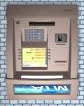
\includegraphics[width=0.85\textwidth]{../../images/python/page_015_img_01.png}

% deskripsi: gambar native xref 136
\noindent
\includegraphics[width=0.85\textwidth]{../../images/python/page_015_img_02.png}

% deskripsi: gambar native xref 137
\noindent
\includegraphics[width=0.85\textwidth]{../../images/python/page_015_img_03.png}

% deskripsi: gambar native xref 142
\noindent
\includegraphics[width=0.85\textwidth]{../../images/python/page_015_img_04.png}

\end{document}
